\documentclass{article}
\usepackage{ctex}
\usepackage[utf8]{inputenc}
\usepackage[T1]{fontenc}
\usepackage{hyperref}
\usepackage{graphicx}
\usepackage[style=numeric,backend=biber,autolang=other]{biblatex} 
\addbibresource{research_ref.bib} % 添加参考文献数据库文件
\setCJKfamilyfont{myfont}{SimSun.ttc}
\newcommand{\SetFont}{\CJKfamily{myfont}}

\title{\textbf{调研报告}}
\author{小组成员: 杨译博,汪睿,张博厚,储\SetFont{溦}}

\begin{document}
\maketitle
\newpage
\tableofcontents
\newpage
% \begin{enumerate}
%     \item  项目概述
%     \item  项目背景
%     \item  立项依据
%     \item  前瞻性/重要性分析
%     \item  相关工作
%     \item  参考文献
% \end{enumerate}
\section{项目概述}
LiteOS 是华为云提供的轻量级物联网操作系统,支持MMU和POSIX接口,适合物联网领域。本项目旨在使用Rust改写LiteOS内核中的内存管理单元,提高其安全性。Rust的接近底层、高性能、安全性使得它可以适于构建操作系统。Rust与C的无缝相互调用的兼容性也为部分改写后接入整体提供了极大的便利。
% \newpage
\section{项目背景}
\subsection{Rust}
\subsubsection{Rust概述}
Rust 是为了解决系统编程领域的安全性问题, 而设计的一门面向系统编程的\textbf{安全可靠、性能出众}的系统级编程语言,具有内存安全性和并发性等特性。近年来,由于其严格的所有权和借用规则,Rust逐渐受到操作系统开发者的青睐,在底层软件系统的构建中得到了越来越广泛的应用。
\subsubsection{编写操作系统的语言}
编写操作系统需要对底层硬件进行直接控制。考虑到标准库依赖操作系统所提供的接口,要编写操作系统,所使用的语言必须要能够不依赖标准库、直接在裸机上运行。除了底层的汇编语言,C、C++、Rust、Pascal都可以满足这一要求。而由于C语言脱离系统的库最丰富和完整、C语言用来开发操作系统的工具最多,当下的大多数操作系统内核都使用C语言。
\subsubsection{Rust的高效性}
作为一门系统级编程语言,Rust的性能与C/C++相差无几\supercite{ref3}。实际上,Rust设计的一个明确目标,就是实现在大部分事情上拥有与C/C++类似的性能。\\
\textbf{系统级编程语言}:在编译时,Rust代码被转化为中间表示,然后经过优化生成目标平台的机器码。生成的机器码直接与底层硬件进行交互。相比于解释型语言,Rust在编译过程中往往花费更多的时间来进行额外编译过程和优化,并换来高性能。\\
\textbf{无垃圾回收(GC)}:Rust引入了基于所有权模型的自动内存管理机制,可以在编译时跟踪程序中资源的变量,并在无GC的情况下完成这些操作。这使得Rust没有必要通过自动垃圾收集等内存管理机制来处理在 C/C++程序中常见的悬空指针、重复释放、空指针引用等内存安全漏洞。避免了GC带来的性能损失。\\
\textbf{零成本抽象}:Rust具有现代编程语言的高级抽象特性,编译器能够在编译时进行零成本抽象,所有的抽象都会在编译过程中被处理,从而避免资源消耗。\\
\textbf{不依赖虚拟机(VM)}:Rust代码经过编译后直接生成本机机器码,在运行时不需要任何虚拟机,可以更高效地利用计算资源,提高性能并降低内存消耗。\\
这些特性保证了Rust的高效性,并使之成为高性能、系统级和嵌入式编程的理想选择。
\subsubsection{Rust的安全性}
Rust的核心语言安全特性\supercite{ref5}使得 Rust在具有可媲美 C/C++的高性能的同时, 实现了类型安全、内存安全和并发安全。\\
\textbf{函数式编程范式}:\\
变量必须被显式初始化且默认不可变,在多线程访问变量时,这保证了程序不必使用加锁等易出错的同步操作,Rust的这一特性有利于构建安全的并发程序。Rust的模式匹配语言特性要求模式匹配覆盖所有分支可能有助于在编译时捕获潜在的错误,并提高代码的安全性。\\
\textbf{强多态类型系统}:\\
Rust使用强类型系统来保证程序的类型安全,并引入多态类型(Trait多态\supercite{ref14}、泛函多态\supercite{ref15})和类型推导来增强静态类型系统的检查能力。\\
\textbf{基于所有权模型的自动内存管理}:\\
所有权模型:变量与存放在内存某块的值绑定,程序的每个值都有唯一的所有者,该值的生命周期局限于所有者的作用范围,离开作用范围后,Rust编译器插入的内存回收语句将回收位置和销毁值。\supercite{ref7}\\
借用和引用:引用机制允许多个不可变引用指向同一个内存单元, 或者唯一的可变引用指向一个内存单元。引用和基于引用的借用机制用于处理所有权模型带来的限制,使程序设计有更多灵活性。\supercite{ref8}\\
所有权、引用和借用等机制使得 Rust具备C/C++等语言不具备的内存安全和并发安全——杜绝了悬空指针、二次释放、空指针引用、释放后使用等隐患, 并且规避了线程间可变变量的共享。\\
\textbf{对非安全代码的显式标记和隔离}:\\
在Rust中,可以使用unsafe关键字来构建非安全代码块(unsafe blocks),从而可以在需要时绕过编译器的严格静态检查,执行一些底层、系统级或涉及不安全操作的任务。Rust编译器不会对非安全代码块可能的5种不安全操作(包括解引用裸指针、调用unsafe的函数或方法、实现不安全的trait、访问或修改可变静态变量的值、读写union 联合体中的字段)进行检查,但此外的安全检查仍然严格执行。\\
Rust对非安全代码的显式标记和隔离允许程序员在必要时使用不安全操作,从而保证了安全性和灵活性的平衡。
\subsubsection{Rust的兼容性}
Rust提供了对C ABI(Application Binary Interface,应用程序二进制接口)的支持,即Rust 可以与C语言进行无缝的集成。Rust可以直接调用C函数,并且可以将Rust函数暴露给C代码使用\supercite{ref16}。Rust与C无需额外的中间层即可互操作,这种良好的兼容性这为Rust改写C语言操作系统提供了方便。并且在这种交互中,Rust的所有权系统和类型系统仍然确保了内存安全性和线程安全性。
\subsection{LiteOS}
\subsubsection{LiteOS简介}
Huawei LiteOS(下简称LiteOS)是华为面向IoT领域构建的\textbf{轻量级物联网操作系统},可广泛应用于智能家居、个人穿戴、车联网、城市公共服务、制造业等领域。LiteOS遵循BSD-3开源许可协议, 目前已支持 ARM64、ARM Cortex-A、ARM Cortex-M0,Cortex-M3,Cortex-M4,Cortex-M7 等芯片架构\supercite{ref4}。
Huawei LiteOS自开源社区发布以来,围绕物联网市场从技术、生态、解决方案、商用支持等多维度使能合作伙伴,构建开源的物联网生态,目前已经聚合了50+ MCU和解决方案合作伙伴,共同推出一批开源开发套件和行业解决方案,帮助众多行业客户快速的推出物联网终端和服务,客户涵盖抄表、停车、路灯、环保、共享单车、物流等众多行业,加速物联网产业发展和行业数字化转型。
\subsubsection{LiteOS的优势}
\noindent
\paragraph{轻量级设计}:LiteOS被设计为一款轻量级操作系统, 内核小巧,占用空间少(基本内核可裁剪至最小10kiB), 因此所需的硬件资源少,适合在资源受限的物联网设备上运行。\\

\paragraph{低功耗}:LiteOS 采用了优化的功耗管理机制,能够有效地管理设备的能量消耗,运行在配套芯片上时可将功耗降低至$\mu A$级\supercite{ref4}。\\
\paragraph{高实时性}:LiteOS的轻量性使得内核运行效率较高,任务调度和切换的开销较小,从而可以降低系统的响应延迟,提高实时性;LiteOS的启动速度与响应速度快, 可以迅速响应各类需求与任务,包括开机、传感器数据的采集、网络通信的处理、用户交互的响应等,做到实时反馈;此外,LiteOS具备高效的任务调度机制,允许用户在其上运行实时任务。这些都使得LiteOS具备高实时性的特点。\\
\paragraph{支持静态功能裁剪}:LiteOS 提供了灵活的配置选项,用户可以根据实际情况对系统进行配置,去除不需要的功能和组件,还可以根据具体的硬件平台和应用场景,优化 LiteOS 的资源配置,包括内存分配、任务优先级设置等,以提高系统的性能和效率。
\subsubsection{架构与设计原理}
LiteOS基础内核包括不可裁剪的极小内核和可裁剪的其他模块。极小内核包含任务管理、内存管理、中断管理、异常管理和系统时钟。可裁剪的模块包括信号量、互斥锁、队列管理、事件管理、软件定时器等。 Huawei LiteOS支持 UP(单核)与 SMP(多核)模式,即支持在单核或者多核的环境上运行。架构图如图\ref{fig:1}所示。

\paragraph{任务管理} \textbf{(a)}LiteOS中以任务(Task)作为内核的基本执行单元(也是资源分配的最小单元),这与传统操作系统中的进程(Process)概念类似,但LiteOS中不具备完整的进程调度机制,每个任务都有独立的任务控制块(TCB)和任务栈,任务之间可以通过共享资源或者消息传递的方式进行通信和协作,不同任务之间的隔离程度较低,通信开销也较小。\textbf{(b)}LiteOS使用基于优先级的抢占式任务调度方式,共有32个优先级,低优先级任务需在高优先级任务阻塞或结束后才能获得调度。对于相同优先级的任务,则采用时间片轮转方式调度。
\begin{figure}[htbp]
    \centering
    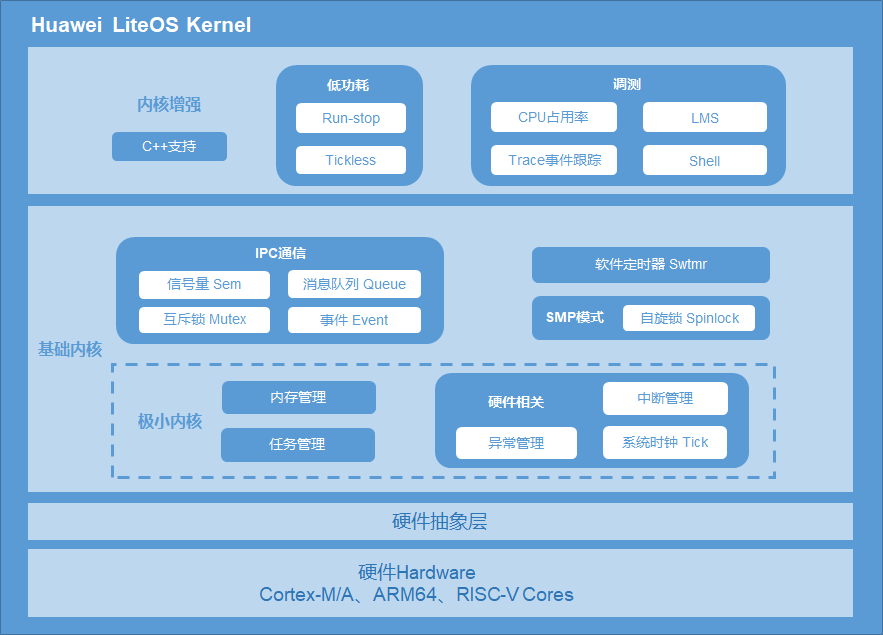
\includegraphics[width = \textwidth]{figs/LiteOS_Kernel_Arch.png}
    \caption{LiteOS内核架构}
    \label{fig:1}
\end{figure}
\paragraph{内存管理} LiteOS的内存管理分为静态内存管理和动态内存管理,提供内存初始化、分配、释放等功能。 LiteOS操作系统将内核与内存管理分开实现,操作系统内核仅规定了必要的内存管理函数原型,而不关心内存管理的函数是如何实现的,所以在LiteOS 中提供了多种内存分配算法(分配策略),但是上层接口(API)却是统一的。这样做可以增加系统的灵活性:用户可以选择对自己更有利的内存管理 策略,在不同的应用场合使用不同的内存分配策略\supercite{ref11}。
\paragraph{中断管理}LiteOS的中断具有如下特性:中断共享,且可配置,依赖链表实现;中断嵌套,即高优先级的中断可抢占低优先级的中断,GIC与NVIC的中断嵌套由硬件实现,RISC-V中的中断嵌套由中断栈实现;使用独立中断栈;可配置支持的中断优先级个数;可配置支持的中断数。
\paragraph{异常接管}异常接管是操作系统对运行期间发生的异常情况(芯片硬件异常)进行处理的一系列动作,例如打印异常发生时当前函数的调用栈信息、CPU现场信息、任务的堆栈情况等。LiteOS的异常接管,在系统发生异常时的处理动作为:显示异常发生时正在运行的任务信息(包括任务名、任务号、堆栈大小等),以及CPU现场等信息。针对某些RISC-V架构的芯片,对内存size要求较高的场景,LiteOS提供了极小特性宏,用于裁剪多余的异常提示字符串信息,但是仍然保留发生异常时的CPU执行环境的所有信息\supercite{ref4}。

\subsection{内存管理单元(MMU)}
\subsubsection{概述}
内存管理单元(MMU)是处理器支持操作系统高效运行的基础,与软件内存管理模块相结合完成了虚拟地址到物理地址的转换。同时,MMU能够对处理器发出的地址进行合法性检验,在硬件上提供了内存访问授权控制。由于MMU与处理器体系结构高度相关,因此在不同的处理器下内存管理机制区别很大。
\begin{figure}[htbp]
    \centering
    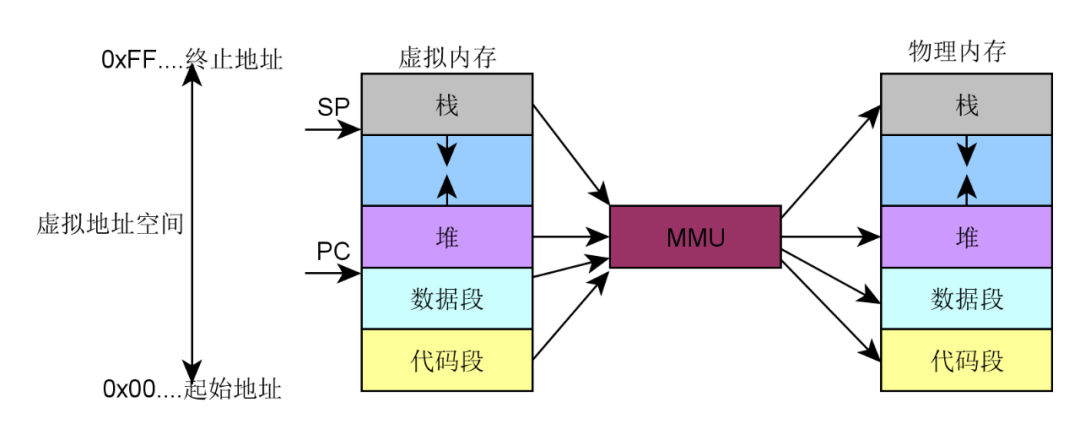
\includegraphics[width = \textwidth]{figs/MMU.png}
    \caption{内存管理单元(MMU)}
    \label{fig:4}
\end{figure}
\subsubsection{内核的内存管理}
为了限制应用访问内存空间的范围并给操作系统提供内存管理的灵活性,计算机硬件需要引入内存保护/映射/地址转换硬件机制,如 RISC-V 的基址-边界翻译和保护机制、x86 的分段机制、RISC-V/x86/ARM 都有的分页机制。如果在地址转换过程中,无法找到物理地址或访问权限有误,则处理器产生非法访问内存的异常错误

% \section{立项依据}
\section{前瞻性/重要性分析}
\subsection{rust重写的意义}
C语言缺少有效的并发支持,导致内存和并发漏洞成为当前操作系统的噩梦。
Rust 语言具有与C一样的硬件控制能力,且大大强化了安全编程。从某种角度上看,Rust 语言的核心目标是解决C的短板,取代C。所以用Rust写liteos具有很好的开发和运行的体验。\supercite{ref12}有时程序员必须执行无法静态验证为安全的操作。Rust 为程序员提供了将这些操作包装在安全抽象的工具中,这意味着Rust编译器可以静态地强制执行那些曾经属于代码注释或约定的操作。
\subsection{rust前瞻}
Rust现有的社区对该语言有巨大的好处。语言的大部分功能来自于其核心之外的库、工具和学习资料。 Rust 仍然是一个年轻的语言,但是它拥有一个健康的生态系统,拥有一个活跃的、开放的编译器和语言的开发过程,并且它显示出了强大的促进开源社区和支持用户生产力的能力。这给了我们更多的理由相信该语言有一个光明的未来。\supercite{ref13}
\subsection{LiteOS横向对比}
大多数的RTOS都是运行于MCU(单片机上),不支持MMU(内存管理单元),内核空间和APP空间不能隔离开,APP出错后整个系统就会崩溃;也不支持POSIX接口,这使得大量的开源软件无法直接在MCU上运行。
\paragraph{内存管理单元 (MMU) 支持}LiteOS 支持 MMU,这意味着它可以实现内核空间和应用程序空间的隔离。这种隔离性能够确保应用程序出现问题时不会影响到整个系统,提高了系统的健壮性和稳定性。
\paragraph{POSIX 接口支持}:LiteOS 支持 POSIX 接口,这使得大量的开源软件可以直接在 LiteOS 上运行。与其他没有 POSIX 接口支持的 RTOS 相比,LiteOS 的生态系统更加丰富,开发者可以更快速地开发应用程序,并且可以利用现有的开源软件资源。
\paragraph{低功耗}通过支持Tickless机制、run-stop休眠唤醒,可以极大地降低系统功耗。
\paragraph{社区支持和未来发展}: 尽管 LiteOS 是相对年轻的操作系统,但它已经拥有了一个活跃的社区和健康的生态系统。与其他闭源或者相对较小的 RTOS 相比,LiteOS 拥有更多的开发者和用户,并且在不断地发展和改进中。这为 LiteOS 的未来发展提供了更多的可能性和机会。
综上所述,与其他常见的嵌入式实时操作系统相比,LiteOS 在支持 MMU、POSIX 接口、启动速度和节能性等方面具有优势,并且拥有一个活跃的社区和健康的生态系统,为其未来的发展奠定了良好的基础。
\section{相关工作}
\subsection{Redox OS}
Redox OS 是一个用 Rust 语言编写的类 UNIX 开源操作系统,其采用微内核架构,与 Linux 宏内核相比,它的体积和使用的基本功能较少,它支持常见的 UNIX 命令,包含 C 程序的新移植库,同时也支持 Rust 标准库,驱动程序运行在用户空间,作为早期开发的基于 Rust 的操作系统,其具有很好的安全性和可用性。
\subsection{Tock OS}
Tock OS 是一个由 Rust 语言编写的嵌入式操作系统,设计用于在基于 Cortex-M 和 RISC-V 的嵌入式平台上运行多个并发的、互不信任的应用程序。Tock 的设计以保护为中心,既可以防止潜在的恶意应用程序,也可以防止设备驱动程序。Tock 使用两种机制来保护操作系统的不同组件。首先,内核和设备驱动程序是用 Rust 编写的,Rust 是一种提供 compile-time 内存安全、类型安全和严格别名的系统编程语言。Tock 使用 Rust 来保护内核(例如调度程序和硬件抽象层)不受特定于平台的设备驱动程序的影响,并将设备驱动程序彼此隔离。其次,Tock 使用内存保护单元将应用程序彼此和内核隔离开来,从而大大提高了系统的安全性。
\subsection{Theseus OS}
Theseus OS 被发表在 OSDI'20,作者来自 Yale 大学和 Rice 大学。Theseus 相比传统的 OS ,采用的思路非常的激进,完全弃用了现有 OS 大多采用的虚拟化和特权等级设计,内存安全则完全由 Rust 语言特性保证。作者用了 PhD 期间几年的功夫独立实现了 Theseus,并用它作为自己的博士毕业论文。\supercite{ref6}

Theseus 试图解决的问题有两个:

1. 系统中常有的 state spill 问题;state spill 是指,如果把某个系统模块看成状态机,它的状态不是自己决定的,而是会在跟其他模块的接触中被改变。这带来的问题是,所有依赖这个模块的其他模块,都会因此共享命运,如果这个模块崩溃了,可能会导致其他所有模块无法使用,因而导致整个系统崩溃。

2. 语言内 OS 设计(intralingual OS design)这是指:让 OS 的运行环境跟实现 OS 用的语言提供的运行时环境相 match。这样就可以尽可能地享受到编译器静态检查带来的便利。

整个 Theseus 系统是由各种各样的 cells 组成的,见\ref{fig:2},每个 cell 负责一个系统功能,并且可以在运行的时候被替换掉。所有的 cell 和用户代码共享同一个地址空间,共享同一个优先级。通过 MMU(内存管理单元)来提供 page 的 RWX 权限管理,整个系统的物理地址一一对应逻辑地址。
\begin{figure}[htbp]
    \centering
    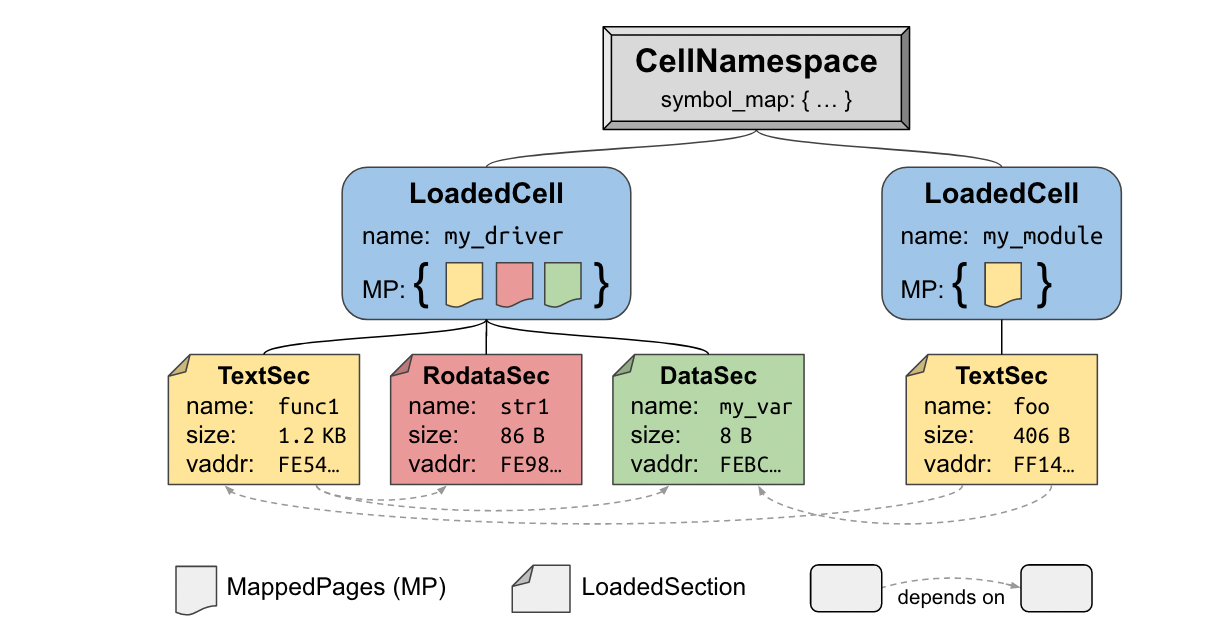
\includegraphics[width = \textwidth]{figs/cells.png}
    \caption{Theseus cell 架构}
    \label{fig:3}
\end{figure}
\subsection{在Linux内核中基于Rust实现的UDP隧道网络驱动程序} 
Amélie Gonzalez ,Djob Mvondo 和 Yérom David Bromberg 三人根据前人将 Rust 语言逐步添加到 Linux 内的经验,如使用 Rust 编写存储设备的驱动程序,设计实现了一个 Linux 下的 Rust UDP隧道驱动程序,\supercite{ref9}它提供了两个节点间的 UDP 封装。但他们发现,与 C 语言编写的驱动程序相比,Rust 驱动程序延迟则增加了近五分之一。
\subsection{基于Rust实现Unikernel}
Stefan Lankes , Jens Breitbart 和 Simon Pickartz 基于Rust语言设计开发了 RustyHermit,\supercite{ref10}它是一个完全由 Rust 编写而不需要 C/C++ 的单核,并且他们还发现对 RustyHermit 的支持可以透明地集成到 Rust 工具链中,并且公共的 Rust 用户程序可以构建在 RustyHermit 上,证明了用 Rust 开发 OS 内核的可行性,
\subsection{C 与 Rust}
几十年来,系统开发一直由诸如 C/C++ 之类的编程语言主导,但这些语言本质上是不安全的,很容易造成系统崩溃,在这样的背景下,具有安全的内存模型的高级编程语言逐渐成为开发者的倾向, Rust 就是最具代表性的语言之一, Rust 的典型特征就是安全性,使用它编写操作系统可以大大提高系统的安全性和运行质量。


Mehmet Emre , Ryan Schroeder , Kyle Dewey 和 Ben Charles Hardekopf 指出,Rust 是一个较新的编程语言,并且他们研究了自动将 C 语言程序转换为更安全的 Rust 程序的问题,并且深究了翻译程序中不安全的潜在原因及修复每个原因的相对影响。\supercite{ref17}

Amit Levy 等人对用 Rust 语言在嵌入式系统中开发操作系统的情况进行了讨论,发现Rust 的所有权模式组织了在嵌入式领域常见的资源共享,与实际情况相冲突,但是他们提出了最大程度上保证安全并且不影响功能的方法,并提出对Rust语言的扩展,以便其能够更好的为内存安全提供工具。\supercite{ref18}



 

%   备注: 利用数据库添加参考文献的使用方法。
%   将文献按照格式添加到research_ref.bib文件中,并在引用该文献的位置使用supercite{文献名}
%   命令,这将会在该处产生上标类型的引用超链接
\newpage
% 比如这样\supercite{ref1}。




\printbibliography[ title = {参考文献}]


\end{document}

